\subsection{Mission de ME~: Réponse technique au stockage des données}
\begin{frame}
	\frametitle{Mission de ME~: Réponse technique au stockage des données}
\end{frame}

% Fonctionnalité de données~:
%% Problématique~: Stockage des données.
%% Solutions possibles~: SGBDR, XML...
%% Solution choisie \& raisons~: SGBDR MySQL (rebondissement Postgres)
%%% Implémentation, problèmes rencontrés (Driver QMYSQL, solution de contournement SQLite...), etc.


\subsection[Nature des données]{Nature des données}
\begin{frame}
\transdissolve[duration=0.2]<1->
\frametitle{Nature des données}
\begin{columns}[c]
\begin{column}{12cm}
\begin{block}{\textbf{Quelle est la nature des données qui vont être stockées ?}}
\begin{itemize}
\item<2-> \textbf{Réquisitions et Waybills}
\item<3-> \textbf{Personnes}
\item<4-> \textbf{Véhicules}
\item<5-> \textbf{Pays}
\item<6-> ...
\end{itemize}
\end{block}
\visible<7>{
$\Rightarrow$ Les données sont donc \textbf{multiples} et de nature \textbf{diverses}.}
\end{column}
\end{columns}
\end{frame}

\subsection[Fonctionnalités de base de données]{Fonctionnalités de base de données}
\begin{frame}
\transdissolve[duration=0.2]<2->
\frametitle{Fonctionnalités de base de données}
\begin{columns}[c]
\begin{column}{12cm}
\begin{block}{\textbf{Quelle sont les fonctionnalités attendues ?}}
La base de données en accord avec les besoins formulés dans le CdC de consultation doit permettre~:
\begin{itemize}
\item<2-> \textbf{Gérer les réquisitions \& waybills/delivery~notes (ajout, modification, supprimer)}
\item<3-> \textbf{Faire un suivi des transporteurs, livraisons et des prestataires de service}
\item<4-> \textbf{Gérer les documents administratifs (permis, assurances, contrats, véhicule...)}
\end{itemize}
\end{block}
\end{column}
\end{columns}
\end{frame}

\subsection[Problématique relative aux données]{Problématique relative aux données}
\begin{frame}
\transdissolve[duration=0.2]<2->
\frametitle{Problématique relative aux données}
Cette problématique est divisée selon trois points clés~:
\begin{itemize}
	\item<2-> \textbf{Le stockage}
	\item<3-> \textbf{Le transfert}
	\item<4-> \textbf{L'importation~/~exportation}
\end{itemize}
\end{frame}

\subsection[Solutions possibles]{Solutions possibles}
\begin{frame}
\transdissolve[duration=0.2]<2->
\frametitle{Solutions possibles}
\begin{columns}
\begin{column}{5cm}
\begin{itemize}[<+->]
	\item<2-> Oracle Database
	\item<3-> PostgreSQL
	\item<4-> MySQL
	\item<5-> Microsoft SQL Server
	\item<6-> SQLite
\end{itemize}
\end{column}
\begin{column}{7cm}

\begin{figure}
\visible<2->{

\includegraphics[scale=0.038]{Images/Oracle}
}\visible<3->{

\includegraphics[scale=0.18]{Images/PostgreSQL}\\
}\visible<4->{

\includegraphics[scale=0.04]{Images/MySQL}\\
}\visible<5->{

\includegraphics[scale=0.052]{Images/MsSqlServer}
}\visible<6->{

\includegraphics[scale=0.052]{Images/SQLite}
}
\end{figure}
\end{column}
\end{columns}
\end{frame}

\subsection[Solution retenue]{Solution retenue}
\begin{frame}
\frametitle{Solution retenue}
\begin{columns}
\begin{column}{5cm}
\begin{itemize}
	\item Oracle Database
	\item PostgreSQL
	\item \textbf{MySQL}
	\item Microsoft SQL Server
	\item SQLite
\end{itemize}
\end{column}
\begin{column}{7cm}
\begin{figure}

\includegraphics[scale=0.038]{Images/Oracle}

\includegraphics[scale=0.18]{Images/PostgreSQL}\\

\includegraphics[scale=0.04]{Images/MySQL}\\

\includegraphics[scale=0.052]{Images/MsSqlServer}

\includegraphics[scale=0.052]{Images/SQLite}
\end{figure}
\end{column}
\end{columns}
\end{frame}

\begin{frame}
\transdissolve[duration=0.2]<2->
\frametitle{Solution retenue}
\begin{block}{\textbf{Pourquoi ce SGBDR ?}}
\begin{itemize}
 \item<2-> \textbf{Interopérabilité maximale avec la solution de l'existant}
 \item<3-> \textbf{Solution ne nécessitant pas de coût lié à la formation}
 \item<4-> Solution pouvant facilement s'interfacer à l'aide d'API diverses
 \item<5-> Traitement rapide des requêtes
\end{itemize}
\end{block}
\end{frame}

\subsection[Modélisation Conceptuelle et implémentation]{Modélisation Conceptuelle et implémentation}
\begin{frame}
\frametitle{Modélisation Conceptuelle}
La modélisation conceptuelle des données a été réalisé à l'aide de l'outil \textbf{JMerise}.\\
\begin{center}
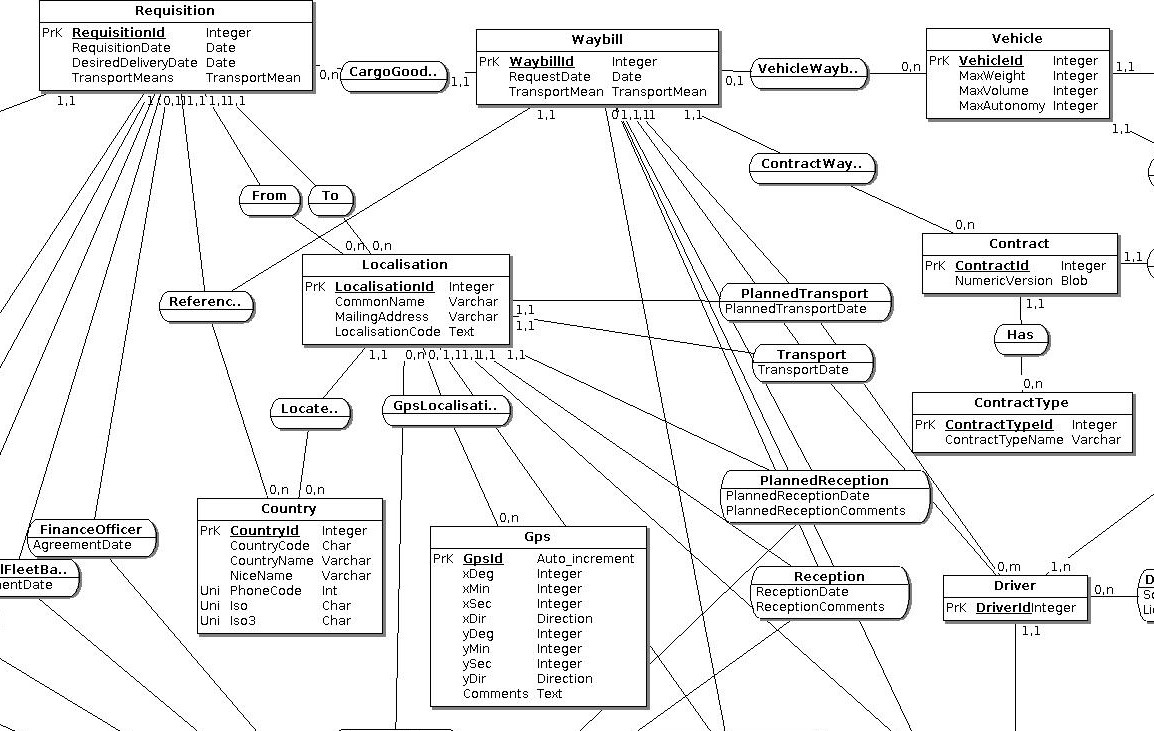
\includegraphics[scale=0.15]{Images/DatabaseSize}
\end{center}
\end{frame}

\begin{frame}
\transdissolve[duration=0.2]<2->
\frametitle{Implémentation}
Le bon fonctionnement de la base de données s'appuie sur les fichiers suivants~:
\begin{enumerate}
	\item<2-> \emph{Database.properties}
	\item<3-> \emph{Database.mcd}
	\item<4-> \emph{Database.sql}
\end{enumerate}
\end{frame}

\subsection[Transfert et import~/~export]{Transfert et import~/~export}
\begin{frame}
\frametitle{Transfert et import~/~export}
Le transfert des données se fait par requêtes SQL.\\
Une représentation XML de la base est présente pour limiter le volume de data par compression.\\
\end{frame}

\subsection{Difficultés rencontrées}
\begin{frame}
\transdissolve[duration=0.2]<2->
\frametitle{Difficultés rencontrées}
Les principaux problèmes ont été~:
\begin{itemize}
\item<2-> \textbf{Conceptualisation et relations entre les tables}
\item<3-> \textbf{Driver QMYSQL pour Qt et migration}
\end{itemize}
\end{frame}
